\documentclass[14pt,a4paper,report]{report}
\usepackage[a4paper, mag=1000, left=2.5cm, right=1cm, top=2cm, bottom=2cm, headsep=0.7cm, footskip=1cm]{geometry}
\usepackage[utf8]{inputenc}
\usepackage[english,russian]{babel}
\usepackage{indentfirst}
\usepackage[dvipsnames]{xcolor}
\usepackage[colorlinks]{hyperref}
\usepackage{listings} 
\usepackage{fancyhdr}
\usepackage{caption}
\usepackage{amsmath}
\usepackage{latexsym}
\usepackage{graphicx}
\usepackage{array}
\hypersetup{
	colorlinks = true,
	linkcolor  = black
}

\usepackage{titlesec}
\titleformat{\chapter}
{\Large\bfseries} % format
{}                % label
{0pt}             % sep
{\huge}           % before-code


\DeclareCaptionFont{white}{\color{white}} 

% Listing description
\usepackage{listings} 
\DeclareCaptionFormat{listing}{\colorbox{gray}{\parbox{\textwidth}{#1#2#3}}}
\captionsetup[lstlisting]{format=listing,labelfont=white,textfont=white}
\lstset{ 
	% Listing settings
	inputencoding = utf8,			
	extendedchars = \true, 
	keepspaces = true, 			  	 % Поддержка кириллицы и пробелов в комментариях
	language = C,            	 	 % Язык программирования (для подсветки)
	basicstyle = \small\sffamily, 	 % Размер и начертание шрифта для подсветки кода
	numbers = left,               	 % Где поставить нумерацию строк (слева\справа)
	numberstyle = \tiny,          	 % Размер шрифта для номеров строк
	stepnumber = 1,               	 % Размер шага между двумя номерами строк
	numbersep = 5pt,              	 % Как далеко отстоят номера строк от подсвечиваемого кода
	backgroundcolor = \color{white}, % Цвет фона подсветки - используем \usepackage{color}
	showspaces = false,           	 % Показывать или нет пробелы специальными отступами
	showstringspaces = false,    	 % Показывать или нет пробелы в строках
	showtabs = false,           	 % Показывать или нет табуляцию в строках
	frame = single,              	 % Рисовать рамку вокруг кода
	tabsize = 2,                  	 % Размер табуляции по умолчанию равен 2 пробелам
	captionpos = t,             	 % Позиция заголовка вверху [t] или внизу [b] 
	breaklines = true,           	 % Автоматически переносить строки (да\нет)
	breakatwhitespace = false,   	 % Переносить строки только если есть пробел
	escapeinside = {\%*}{*)}      	 % Если нужно добавить комментарии в коде
}

\begin{document}

\chapter{Домашнее задание №7}

\subsubsection{Бояркин 43501/3}

\section{Прохождение случайного процесса через динамическую систему}

Пусть дана линейная система с передаточной функцией $W(p)$ и функцией веса $\omega(t)$:

Выходной сигнал:

\begin{figure}[h!]
	\centering
	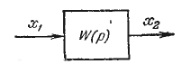
\includegraphics[scale = 0.79]{images/1.png}
	\label{image:1}
\end{figure}

Мат.ожидание:

\begin{figure}[h!]
	\centering
	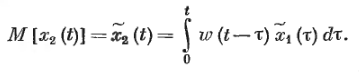
\includegraphics[scale = 0.79]{images/2.png}
	\label{image:2}
\end{figure}

Дисперсия на выходе:

\begin{figure}[h!]
	\centering
	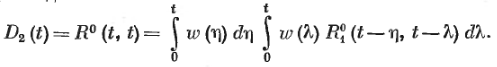
\includegraphics[scale = 0.79]{images/3.png}
	\label{image:3}
\end{figure}

Для установившегося стационарного процесса можно исходить из известной спектральной плотности $S_1(\omega)$:

\begin{figure}[h!]
	\centering
	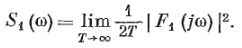
\includegraphics[scale = 0.79]{images/4.png}
	\label{image:4}
\end{figure}

\begin{figure}[h!]
	\centering
	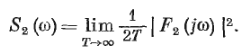
\includegraphics[scale = 0.79]{images/5.png}
	\label{image:5}
\end{figure}

\begin{figure}[h!]
	\centering
	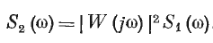
\includegraphics[scale = 0.79]{images/6.png}
	\label{image:6}
\end{figure}

Тогда для нахождения дисперсии интегрирует по всем частотам спектральную плотность:

\begin{figure}[h!]
	\centering
	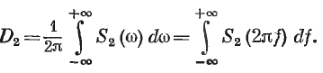
\includegraphics[scale = 0.79]{images/7.png}
	\label{image:7}
\end{figure}

Стоит отметить, что закон распределения для случайной величины при прохождении через линейную систему может меняться. Однако, в случае, если имеем нормальное распределение входной величины, на выходе тоже будет иметь место нормальное распределение.

\clearpage

В общем случае для устойчивой системы нахождение дисперсии можно свести к вычислению:

\begin{figure}[h!]
	\centering
	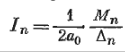
\includegraphics[scale = 0.79]{images/8.png}
	\label{image:8}
\end{figure}

\begin{figure}[h!]
	\centering
	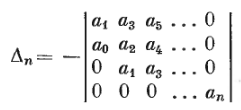
\includegraphics[scale = 0.65]{images/9.png}
	\label{image:9}
\end{figure}

\begin{figure}[h!]
	\centering
	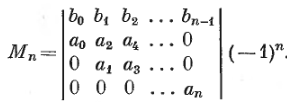
\includegraphics[scale = 0.65]{images/10.png}
	\label{image:10}
\end{figure}

\subsubsection{Статистическое дифференцирование}

При поступлении случайного сигнала на идеальное дифференцирующее устройство с передаточной функцией $W(p)=p$ спектральная плотность выходной величины (производной от входной величины) может быть получена умножением спектральной плотности входной величины на $\omega2$:

\begin{figure}[h!]
	\centering
	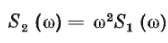
\includegraphics[scale = 0.79]{images/11.png}
	\label{image:11}
\end{figure}

\subsubsection{Статистическое интегрирование}

При поступлении случайного сигнала на идеальное интегрирующее устройство с передаточной функцией $W(p)=1/p$ спектральная плотность выходной величины (интеграла от входной величины) может быть получена делением спектральной плотности входной величины на $\omega2$:

\begin{figure}[h!]
	\centering
	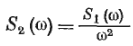
\includegraphics[scale = 0.79]{images/12.png}
	\label{image:12}
\end{figure}

\section{Точность систем управления при случайных воздействиях}

Динамические ошибки при описании входного сигнала детерминированными функциями $g(p)$ в установившемся режиме определяются по формуле: 

\begin{figure}[h!]
	\centering
	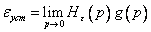
\includegraphics[scale = 0.90]{images/13.png}
	\label{image:13}
\end{figure}

\begin{figure}[h!]
	\centering
	
\includegraphics[scale = 0.90]{images/14.png}
	\label{image:14}
\end{figure}

$H(p)$ - передаточная функция разомкнутой САУ. При описании входного сигнала реализациями случайного процесса $g_0(t)$ динамические ошибки характеризуются величиной дисперсии:

\begin{figure}[h!]
	\centering
	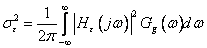
\includegraphics[scale = 0.90]{images/15.png}
	\label{image:15}
\end{figure}

где $G_g(\omega)$ - энергетический спектр входного сигнала $g_0(t)$ . При наличии детерминированных $m(t)$ и случайных $g_0(t)$ составляющих входного сигнала $g(t)=m(t)+g_0(t)$ величину динамических ошибок целесообразно оценивать средним квадратом суммарной ошибки $\epsilon_{ust}^2+\delta^2$.  

Кроме динамических, в САУ имеются ошибки, вызванные действием помех $n(t)$. Влияние помех можно характеризовать дисперсией выходного сигнала САУ:

\begin{figure}[h!]
	\centering
	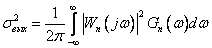
\includegraphics[scale = 0.90]{images/16.png}
	\label{image:16}
\end{figure}

где $W_n(j\omega)$ - передаточная функция по помехе, $G_n(\omega)$ - энергетический спектр помехи. Как правило, помехи в САУ могут быть представлены белым шумом с постоянным на всех частотах энергетическим спектром $G_n(\omega)$. Кроме того, помехи часто действуют на вход системы и тогда передаточная функция по помехе $W_n(j\omega)$ совпадает с передаточной функцией замкнутой САУ:

\begin{figure}[h!]
	\centering
	
\includegraphics[scale = 0.90]{images/17.png}
	\label{image:17}
\end{figure}

Во всех современных САУ присутствуют как динамические ошибки, так и ошибки за счет действия помех. Для характеристики качества системы управления при наличии динамических и случайных ошибок используют средний квадрат суммарной ошибки: 

\begin{figure}[h!]
	\centering
	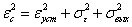
\includegraphics[scale = 0.90]{images/18.png}
	\label{image:18}
\end{figure}

который зависит от параметров $\bar{a}=(a_1, a_2, ..., a_m)^T$ системы. Параметры $\bar{a}$ обычно выбираются таким образом, чтобы обеспечить условие минимума квадрата суммарной ошибки $min_{\bar{a}}\epsilon^2$. В этом случае говорят об оптимизации параметров системы управления по критерию минимума квадрата суммарной ошибки.

Точность систем управления определяется видом входных воздействий и построением самой системы. С точки зрения минимальных установившихся ошибок важную роль играют астатические системы, т.е. системы управления с интеграторами. Наконец, действие помех связано с появлением случайных ошибок, которые оцениваются величиной их дисперсии $\delta^2$ на выходе системы управления.

\end{document}